\chapter{Design}

Tactile vector based devices are inexplored in the HaptiQ (right?) research, our aim is to provide some feedback on their usage for graph exploration. Yet, the key point is to design a device that is affordable and easily reproducible. Our design path also expects to reach the open-source community in order to promote/pave the way for/encourage further contributions.

In this chapter, I will present the device and its functionalities and discuss the different choices that have been made in order to build a functional prototype for our research.

\section{General design}\label{global-design}

The HaptiQ can be seen as a movable device with tactons to aid graph exploration. These tactile feedback is given by actuators on the top of the device forming a star shape. They are directly linked to the hands. Moving the device is an input data provided by the user, just as if we were to move a mouse. This motion is then tracked and processed by a
software layer that will trigger a certain tactile signal, called tacton. The device will lift the actuators up and down according to this tacton signal. (<<< abandoning as per Tigrou's request>>>)

This is how the HaptiQ itself works and the software must meet its
requirements. We can also go beyond these first requirements and provide
a standard API for interaction to be integrated into the software
allowing one interaction to be loaded from a list. Such a software
Although this is the main workflow for the HaptiQ, we do want to be able
to compare this interaction to other techniques. This is why special
efforts have been made for the software part that I will detail.

The feelings that the users experienced by using this device -- the
tactons -- have a direct impact on the usability of the whole system.
Human Computer Interactions (HCI) skills have been applied in order to
make sure that the final tactons are suited for the task of graph
exploration.

Although important, these tactons are supported and limited by the
hardware.

\begin{figure}[!ht]
  \centering
  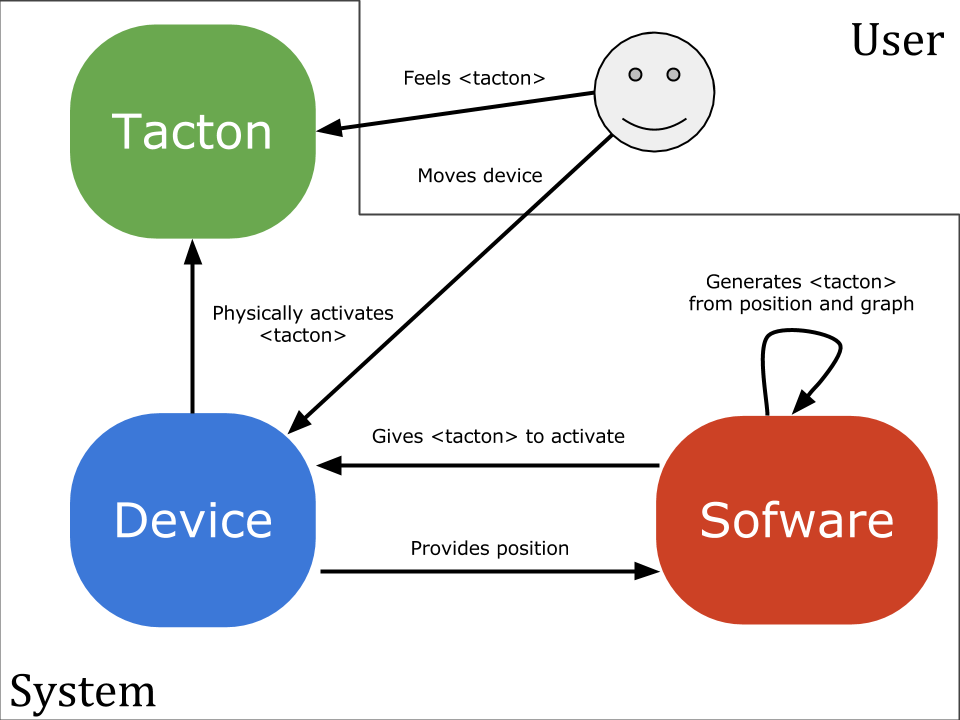
\includegraphics[height=7cm]{figures/haptiq_global.png}
  \caption{Global representation of the HaptiQ project, we have a system and the user}
\end{figure}

\section{Hardware}\label{design-of-the-hardware}

\subsection{Case}\label{case}

The HaptiQ receives the tacton signal to execute. It requires an electronic card connected to the servomotors. In order to be able to move around all this equipement a case is needed and it has to be big enough to encompass everything inside. The first design suggested by Hoggan Eve in Figure TODO made possible to fit everything inside. 

The massive size has actually raised some concerns, but the size aspect is mainly a question of convenience. A second version of the case has been designed by Eve, but the timing was too short in order to guarantee a risk free transfer which was really unfortunate.

\subsection{Electronic components}

The purpose of the HaptiQ is at first, to lift actuators up and down. Although it may seem sufficient, we have faced the possibility to add other interactions like a central button and further interaction like a piezo that plays sounds or vibration. These extra features could be of great value if mixed intelligently with the tactons and it would not have been missing the point to make some time to have them. But our first goal was to understand the tactons, not necessarily use them already and this is why we have decided to leave the button and the vibrations for a later version.

\subsection{Actuator element}\label{actuator-element}

They were two ways of seeing the amount of required elements problem. On one way, it would have taken less time to build a device with four actutors instead of eight and limiting the amount of actuators could have meant to actually increase the efficiency of understanding the activated tacton. On the other hand, we reduce by two the amount of information we can provide when on a node. Besides, we wanted a device that would allow to easily navigate from nodes to nodes and rarely the graphs are fully based on squared angles. Finally, the previous work Simone has done made us prefer this path of development.

\section{Software}

The first version of the application was made with the purpose of building easily tactons (see annexe 1). When the project reached a point where tactons had only minor changes from an iteration to another, I have updated the software.

The second version was intented to be more flexible. The main idea was to provide a software for which most of the parts are easily replacable. This typically has led to a usage of multiple threads. One was to render visually the network, the position and the current tactons; it is called the view. Another provides a position from a communication protocol (TUIO), if we were to replace the source providing the position no change is needed in the software. If we were to change the way we render the position, then only this thread needs to be updated. A last thread handles the execution of the current interaction, for the HaptiQ the interaction is to generate the appropriate tacton and to tell the device to execute it - but other interactions can be used and their executing would have other output. Having this thread executing the current interaction makes it easily adapted for these other interactions. It is also from this second version that I have adapted the code to be cross-platform and added a quick installation guide. This was a way to meet a first basic requirement for a hypothetic larger scale usage.

\section{Tactons}

\subsection{First iteration of
tactons}\label{first-iteration-of-tactons}

In order to understand how tactons work, we have to explain for which
contexts they apply. Here are the following states that are considered
for our tactons:

(figure on node)

(figure on link)

(figure near)

(figure on nothing)

My first iteration has proven me the good distinction between static and
oscillations and that an actuator should guide one graph element. I also
had to find a way of rapid prototyping a usual `paper design' is not
possible with tactile signals.

The possibilities are incredibly wide and any of the ideas I could come up with would have a theory justification. I wanted to have in-use observations as soon as I was able to produce tactons from the software. This first iteration has been evaluated by walkthrough on a visual feedback the 8th of
April 2015 \footnote{\url{https://github.com/asiegfried/vegham/tree/v0.1/app}}. Three participants were asked to find the nodes without being explained the tactons. After some wondering, they were then told how they worked and asked to retry the exploration. I have then invited them to talk about these tactons and encouraged new ideas. They have actually found the nodes by chance, because the oscillation stoped and not because they felt guided towards nodes.

To allow my participants to receive the tacton information, I have decided to represent visually the state of each actuator as shown in Figure FIGURE - the
darker, the higher. This has resulted in a relatively low fidelity
prototype of my set of tactons, yet it is sufficient to observe basic
usability problems. I have had to find my alternative of low fidelity
prototyping and this is how the visual representation has been endorsed.

Because of the early version of this interaction, links were not
integrated yet. The tactons to be generated depended on the following
rules:

\begin{itemize}
\item
  near a node, the tacton indicates the closest nodes by up and down
  oscillations. Actuators moved this way are the two closest angles, so
  if the node is at 40°, the North (90°) and the East (0°) actuators
  gets moved.
\item
  on a node, the tacton indicates the closest nodes by being fully up.
  The concerned actuators are the same as previously.
\end{itemize}

The intention in this set of tactons was to encode as much information
as possible. By using this perticular set of tactons, one would know
when he would be near a node because the oscillations would begin; at
the same time you would still know about nearby nodes. You could easily
distinguish when you are on a node

That was in theory, while experimenting roughly with my low fidelity
feedback, the subjects were feeling lost during the whole exploration
process inspite of me showing where were the ndoes. The following
interviews have revealed the reasons:

\begin{itemize}
\item
  there was far too much information at a giving time
\item
  the interactions felt unatural
\item
  it was impossible to tell how many nodes were nearby
\end{itemize}

Although this interaction was highly depreciated, the task of know
whetether or not we were on a node or not was done accurately. A first
contribution from this first iteration is the efficient distinction
provided by static versus oscillation. This characteristic has been
preserved through the versions. A second one would be the fact that
having more than one actuator guiding a single node was too complex too
be easily processed by the user. This aspect has been taken into account
in the next iterations.

\subsection{Second iteration of
tactons}\label{second-iteration-of-tactons}

The second iteration has brought me consider simple tactons first and
high contrast could be one of the most important characteristic I was
looking for.

Another path was explored from my first iteration, I have tried to find
simpler tactons that could still provide guidance \footnote{\url{https://github.com/asiegfried/vegham/tree/v0.2/app}}.
The following rules concern this second iteration:

\begin{itemize}
\item
  near a node, the tacton indicates the direction towards it with a
  certain intensity. Only one actuator is moved for this tacton, it is
  the one closer to the angle. For instance for a node at 40° it will be
  just the East (0°) actuator. The intensity is inversly proportional to
  the distance. The closer, the higher the level would be.
\item
  on a node, all the actuators are higher than normal.
\end{itemize}

This interaction takes into account what has been remarked in the first
iteration. One actuator is for one node. Oscillation were reserved
purposely for the links, that have not been integrated to the software
at that time.

Another walkthrough has been tried on this interaction in order to
detect usability errors and just in general seeking other ideas. Three participants were asked to find the nodes and to then redraw them on a paper.
This interaction has received several positive feedbacks. The sudden change
for when the pointer is on node makes the message very clear. The
growing intensity also indicated well the exploration. The major issue
remained the fact that these tests were based on visualisation as a
proxy of what the tactile sensations would be. Obviously these two
senses cannot be considered equivalent for my tactons; I had then
reached a limit for my low fidelity prototyping.

Yet, I have understood that simpler is generally better when it comes to
provide guidance. This aspect has motivated my further interaction. The
major contribution of this iteration has been the importance to keep a
clear contrast between the two situations: on node and not on a node.
Since the major difficulty is to find the network, it must be very clear
for the user when it is over a node or not. It accentuates a mental
marker on that very specific zone, it is also reasuring to have such a
clear and distinct tactile feedback.

\subsection{Final generation of
tactons}\label{final-generation-of-tactons}

A few other tactons have been developed while waiting the HatpiQ to be
build. After some hardware issues (that will be presented in
Implementation), I was able to provide the real sensation of the HaptiQ
and this was highly valuable in order to seek the features that would
lead to a suitable tactons.

After several tries through the hardware capacities and my self
judgment, I came up with a last generation of four sets of tactons. The
goal was to compare them in a user study and being able to justify the
most appropriate one for graph exploration. During the first tries out
of this user study, I had to withdraw two of them as they appeared to be
completely unusable for the required task. Two of my collaborators, one
visually impaired one not have experienced the same struggles in using
some of these tacton sets. Among other issues, the users felt
overwhelmed with the tactile information - like arriving on a node, all
the actuators were moving at the same time. And also, it appeared that
the intensity that felt like an interesting idea in the second
iteration, turned out to be completely unperceptable in the real
situation. We can sum up that the main reason why they were not
efficient is because of their lack of simplicity and consistency. I had
to remove them in order to focus on the most promising ones.

The two remaining tacton sets are the result of an iterative exploratory
and are to be compared in a usability study. One can be considered as a
direct mapping of the underneath situation when the second provides an
additional guidance.

\subsubsection{Mapping}\label{mapping}

This tacton sets simply encodes into tactile feedbacks what is directly
underneath the device. It has been narrowed to three very strict rules:

\begin{itemize}
\item
  on a node, the actuators which direction corresponds to the direction
  of a connected node are up, the rest are down.
\item
  on a link, the actuators which direction are parallel to the direction
  of the link are oscillating up and down on an high level, the rest are
  left down.
\item
  on nothing, all the actuators are down.
\end{itemize}

When moving the device onto a node, some actuators goes from a down
level to a up level: their is a high contrast between these two tactile
situations which respects the criteria of a high contrast found during
the second iteration. We have also made good usage of the duality of
static versus oscillation as they both encode distinct facets of the
exploration. Static is for the nodes and emphasize on pausing and maybe
remembering this perticular point. Whereas, oscillations are for
travelling between nodes and this constant feedback of the direction to
go can be seen as an encouragment to proceed.

\subsubsection{Guidance}\label{guidance}

Very close to the previous set of tactons, Guidance offers just one more
rule in order to help keeping track of the network.

\begin{itemize}
\item
  on a node, the actuators which direction corresponds to the direction
  of a connected node are up, the rest are down.
\item
  on a link, the actuators which direction are parallel to the direction
  of the link are oscillating up and down, the rest are left down.
\item
  near a link, the one actuator which direction is the closest to which
  the link is, oscillates in a low level.
\item
  on nothing and near nothing, all the actuators are down.
\end{itemize}

Just as the Mapping set, this one respects the criteria established
during the two previous iterations: high contrast and static versus
oscillation for two different exploration phases. It includes a quick
guidance that helps user to return quickly on their track. Even though a
new tacton is used, the help provided can be worth it. The questions
rised by this alternative are untangled in the Evaluation chapter.

\subsection{Remarks}\label{remarks}

As one would notice, the sets have
been constantly moving towards simplicity and contrast. One can argue
that providing guidance is obviously more usable, but since the
beginning of my internship I have been surprised by the difficulty of
finding the key elements for a good tactile sensation. I have not taken
this for granted and this is why I felt the user study is justified.
Besides, providing some analyse feedbacks on the differences of mapping
versus guidance can surely be seen as a minor contribution in the
understanding of tactile feedback based on vector for graph exploration.
We may appreciate the fact that, as an engineer it is easy to see many
different ways to encode in tactons the underneath situation of a
pointing device. As challenging as it seems, this approach does not
consider the usability aspect.

This chapter has described the design of the software, the tactons and
the hardware. Furthermore, it has detailed the reason of the iteration
over some of them. We end up having a relatively inexpensive device -
around \euro{300} and reproductible. The software is opensource and
using the HaptiQ interactions is cross-platform; it is even designed to
welcome new interaction techniques for the device or to ease comparison.
The implementation of this design has lead to some rationale desicions
as well which will be detail in the Implementation chapter.
